\subsection{How Often Does an Averaged Model Recapitulate Averaged Measurements?}
In the section data-sources, I show that some of the NeuroElectro data distributions look bi-modal. Especially when looking closely at the olfactory mitral cell. In the worst case using the fitting to the mean of a bi-modal distribution might be like fitting a modal to data, that is hard to fit, because its not representative of a real cell. Neuron modellers have some awareness of this problem which has been thoroughly characterized in \cite{marder2011multiple}.

For a selection of three model measurements: we are interested in the question: ``Could misrepresented data, lead to a situation were models cannot match  misconstrued targets?" %We were interested in the consequence of this worst case. 

I placed two different versions of the same  model class in different locations of parameter space. For each location I measured: rheobase, input resistance, capacitance, and membrane time constant.
I then averaged these measurements together to obtain a mean set of electrical measurements, its this collection of measurements that I refer to as ``mean measurements". Next we created a ``mean model' by averaging the locations in parameter space together.
In averaging between two points we create a third point that is midway between the pre-existing coordinates. I refer to the third midway point as a "mean-model".
The mean model is used to create a third set of model measurements, as we are really interested in the question: "Does the mean model sometimes fail to recapitulate the mean measurement?"


%With these different parameter sets we took separate measurements of the listed electrical properties, 
When we have mean measurements, and also mean model measurements, by showing that the two are unequal, we are able to argue that the bi-modal distributions of measurements in experimental data can and do misguide the  optimization of models.

Previously in methods \ref{section:nelectro}, we  inspected the NeuroElectro data sources closely, in order to assess each measurements distribution.
We revealed Bi-modal distributions in input resistance, and cell membrane capacitance, but we do not yet know if it is invalid to fit to the mean of a bi-modal distribution.
Consider a  cell class which had an underlying bimodal distribution for input resistance. An individual cell from this class produced measurements for input resistance midway between two modes for input resistance.
Its entirely conceivable that that this mean cell would produce measurements that were also the mean of the two modes, however, we cannot assume that there this to be true, it seems equally likely that this midway cell produces a measurement for input resistance, that is significantly higher or lower than the mean of the two modes. To bolster that this non linear behavior could be a problem with in-silico models of in-vivo experiments.
We created virtual experiments to expose non-linear behavior between two  close, but different sets of model parameters.

%set about establishing that it is a problem in modelling space.
%The genetic algorithm approach, of recombining model parameters to sample error surface is a similar concept. We do not naively interpolate using midway points, becuase we don't expect that small changes in model parameters to have linear effects.
%to sampling models 

We expect the Izhikevich model, and the adaptive exponential models to support ``regime" change, that is we know that there are regions in parameter space that where when entered cell behavior becomes fundamentally different. For instance in the Izhikevich model, some regions support tonic-bursting and other regions support chattering. 

\begin{figure}
    \centering
    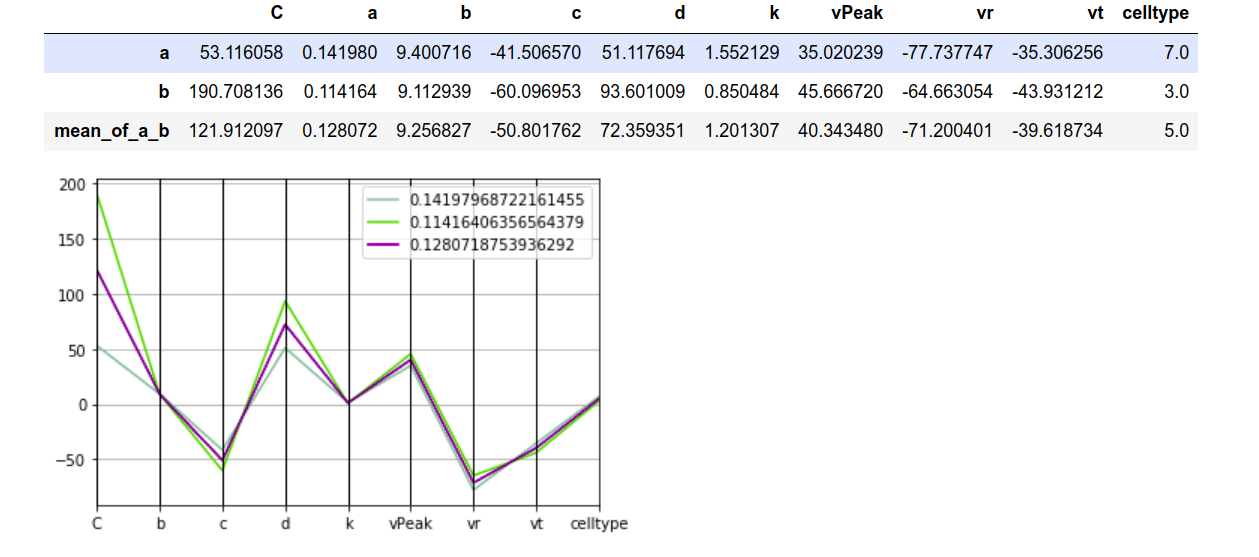
\includegraphics{figures/mean_model_mean_measure_ment_params.png}
    \caption[sets of coordinates that describe three different points in parameters space]{A table of the three different locations in parameter space, each of the coordinates is listed in the table as \textbf{a},\textbf{b}, \textbf{mean-of-a-b}. Beneath the table is a parallel coordinates plot, which makes differences in proportion more clear}
    \label{fig:my_label}
\end{figure}

%\begin{figure}
%    \centering
%    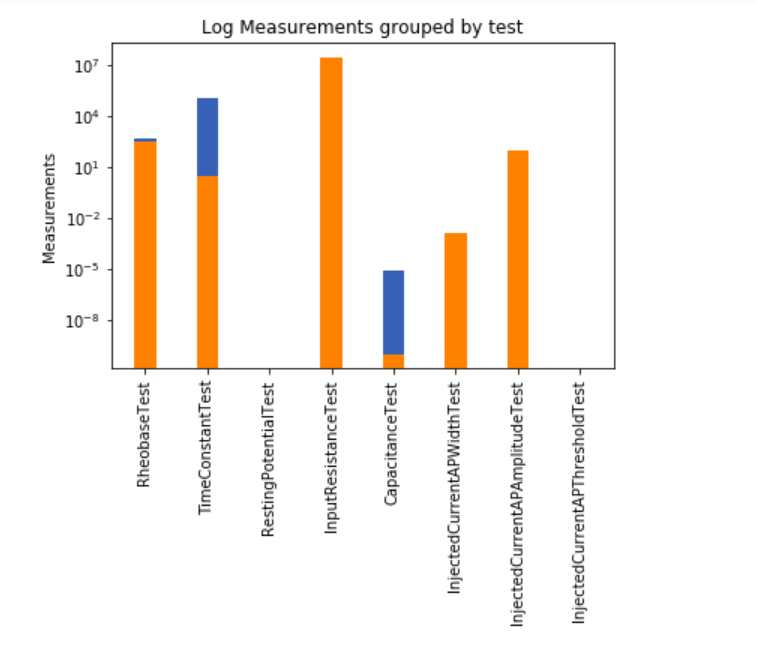
\includegraphics{figures/mean_model_mean_test.png}
%    \caption{Caption}
%    \label{fig:my_label}
%\end{figure}

\begin{figure}
    \centering
    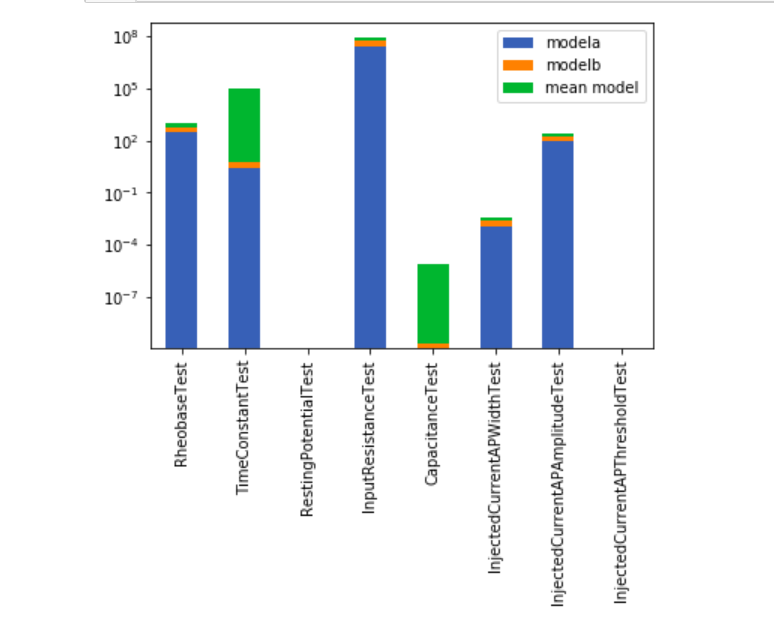
\includegraphics{figures/mean_model_mean_test2.png}
    \caption[bar charts that reveal disparity between mean model and mean measurement]{A stacked bar chart was used and each bar was positioned to represent each of the different measurement types. Very often the mean model measurement, green, is at a comparable height as model a, b and the mean model. There are two glaring exceptions which are the time constant measurement, and the time constant measurement. At those measurement locations the mean is significantly greater than the mean of model a and model b}
    \label{fig:my_label}
\end{figure}

%explore if this was a problem for models as well as experimental cells.